% -*- root: ../main.tex -*-
\chapter{Optymalizacja matematyczna}
\label{chap:optimization}

Optymalizacja matematyczna jest dziedziną rozpoczynającą się od największych nazwisk w matematyce, m.in. Newton i Gauss odkryli pierwsze iteracyjne metody poruszania się w stronę optimum, a Fermat i Lagrange znaleźli sposoby wynikające z rachunku różniczkowego na znajdywanie tych maksimów i minimów. Innym ważnym nazwiskiem dla dziedziny jest Dantzig, który stworzył algorytm Simplex, myląc \break nierozwiązany problem z zadaniem domowym. Mimo iż optymalizacja ma długi rodowód, to nadal jest rosnącą dziedziną z wieloma osobliwościami. Obecnie wykorzystuje się w niej zaawansowany aparat matematyczny, który pozwala na tworzenie lepszych metod optymalizacyjnych. Rozwiązania z tej dziedziny są wykorzystywane w mechanice do projektowania budynków czy przedmiotów, w ekonomii do modelowania zachowań ludzi czy też w elektrotechnice. Widzimy więc, że dziedzina ta istniała przed powstaniem sztucznej inteligencji i posiada wiele zastosowań. My spojrzymy na nią w wymiarze, w którym pozwoli nam ona osiągnąć, to czego potrzebujemy do działania naszych systemów oraz pokażemy kluczowe pomysły. Należy jednak zaznaczyć, że większość ludzi pracujących w AI używa bibliotek, które zawierają znane, najlepsze wersje optymalizatorów. Jednak aby stosować opisane metody z sukcesem, kluczowym jest zrozumienie wewnętrznego działania tych technik.\newline

Podstawowym pomysłem stojącym za użyciem metod optymalizacyjnych w AI jest to, że często mamy rozległy zasób możliwości, z którego nie potrafimy w jasny sposób wybrać najlepszej możliwości bez ekstensywnej eksploracji. Pomyślmy np. o wyborze dania w restauracji szybkiej obsługi. Chcemy wybrać jedzenie do 500 kcal, które będzie nam najbardziej smakowało. Moglibyśmy np. zjeść BigMac’a, który ma 495 kcal i wyczerpuje za jednym razem cały nasz limit, jednak równie dobrze możemy wybrać małe frytki, mały shake i sos jogurtowo-koperkowy co sprawi, że zmieścimy się w limicie tym razem z 485 kcal. Takich możliwości jest naprawdę dużo. Zamiast sosu moglibyśmy wziąć, chociażby kawę albo zamiast shake’a dużą colę. W takich przypadkach przydaje się znajomość technik optymalizacji. Pozwalają nam one na przetestowanie dużej liczby możliwości i wybranie takiej, która najbardziej nam odpowiada. Do tego problemu powrócimy później. Zazwyczaj jednak skupiamy się na sytuacjach ciągłych, w których możemy wybrać dowolną ilość danej rzeczy. To tak jakbyśmy mogli zamówić 1,2 frytek lub 0,56 sosu. Ponieważ zazwyczaj restauracje nie pozwalają nam na taką ekstrawagancję, to skupimy się na trochę innym przykładzie. Pomyślmy o sytuacji, w której chcemy wybrać najlepsze miejsce na wybudowanie domu. Oczywiście w teorii możemy uszeregować wszystkie dostępne miejsca i wybrać najlepsze, ale może być takich możliwości nazbyt wiele. Moglibyśmy przecież postawić nasz dom nad morzem lub w górach, na obrzeżu miasta lub w wiosce, na płaskim lub nierównym terenie, w końcu na skale lub na piasku. Ponieważ nie jesteśmy w stanie sprawdzić wszystkich tych możliwości, ze względu na ich ilość, to z pomocą przychodzi nam optymalizacja matematyczna. Odpowiada ona na pytanie: jaki jest najlepszy sposób, aby badać tę przestrzeń możliwości? Nasza przestrzeń ma pewną korzystną właściwość, a mianowicie może być opisana matematycznie. Jeśli weźmiemy pod uwagę położenie domu na mapie, to otrzymujemy przestrzeń kartezjańską z zaznaczonymi na niej punktami, które odzwierciedlają możliwe położenie domu. Mamy więc dwie potrzebne rzeczy dla optymalizatora, a mianowicie przestrzeń oraz możliwe położenia do testowania. Brakuje nam jednak jeszcze jednego. Metoda, której użyjemy, musi wiedzieć, jak bardzo cenimy dane położenie, aby być w stanie dać nam coraz to lepsze rezultaty. Tak więc załóżmy, że dla każdego pojawiającego się położenia będziemy wpisywać wartość ręcznie. Z takim przygotowaniem możemy użyć metod optymalizacyjnych. Jak to będzie działać? Jeśli poruszymy się, powiedzmy w pierwszym kroku w stronę morza, a my wolimy góry, to przypiszemy nowemu położeniu niższą wartość. Optymalizator sam ‘zorientuje się', że należy kierować się w przeciwnym kierunku i w następnych krokach zmieni sposób poruszania się.

\section{Metoda prób i błędów}

Spróbujemy teraz sformalizować, to co opisaliśmy w poprzednim podrozdziale. \break Możesz nadal myśleć o wyborze najkorzystniejszego położenia na dom, nie będzie to kolidować z formalną definicją. Problem jest określony następująco: Mamy zmienną $\boldsymbol{y}$ którą chcemy optymalizować, to znaczy sprawić, aby była jak największa. Zmienna $\boldsymbol{y}$ zależy od zmiennej $\boldsymbol{x}$ w jakiś nieznany nam sposób. Jednak możemy wpływać na $\boldsymbol{x}$ poprzez podejmowanie akcji. Wyobraźmy sobie, że możemy go zmieniać, tak jak zmienialiśmy położenie domu.\newline

\begin{equation}
max(y = f(x))
\end{equation}

Gdzie $\boldsymbol{x}$ jest zmienną, na którą mamy wpływ, $\boldsymbol{f}$ jest transformacją, której zazwyczaj nieznamy, \textbf{max(y)} mówi nam, że $\boldsymbol{y}$ jest celem, inaczej mówiąc wielkością, którą chcemy maksymalizować.\newline

\clearpage
\begin{figure}[H]
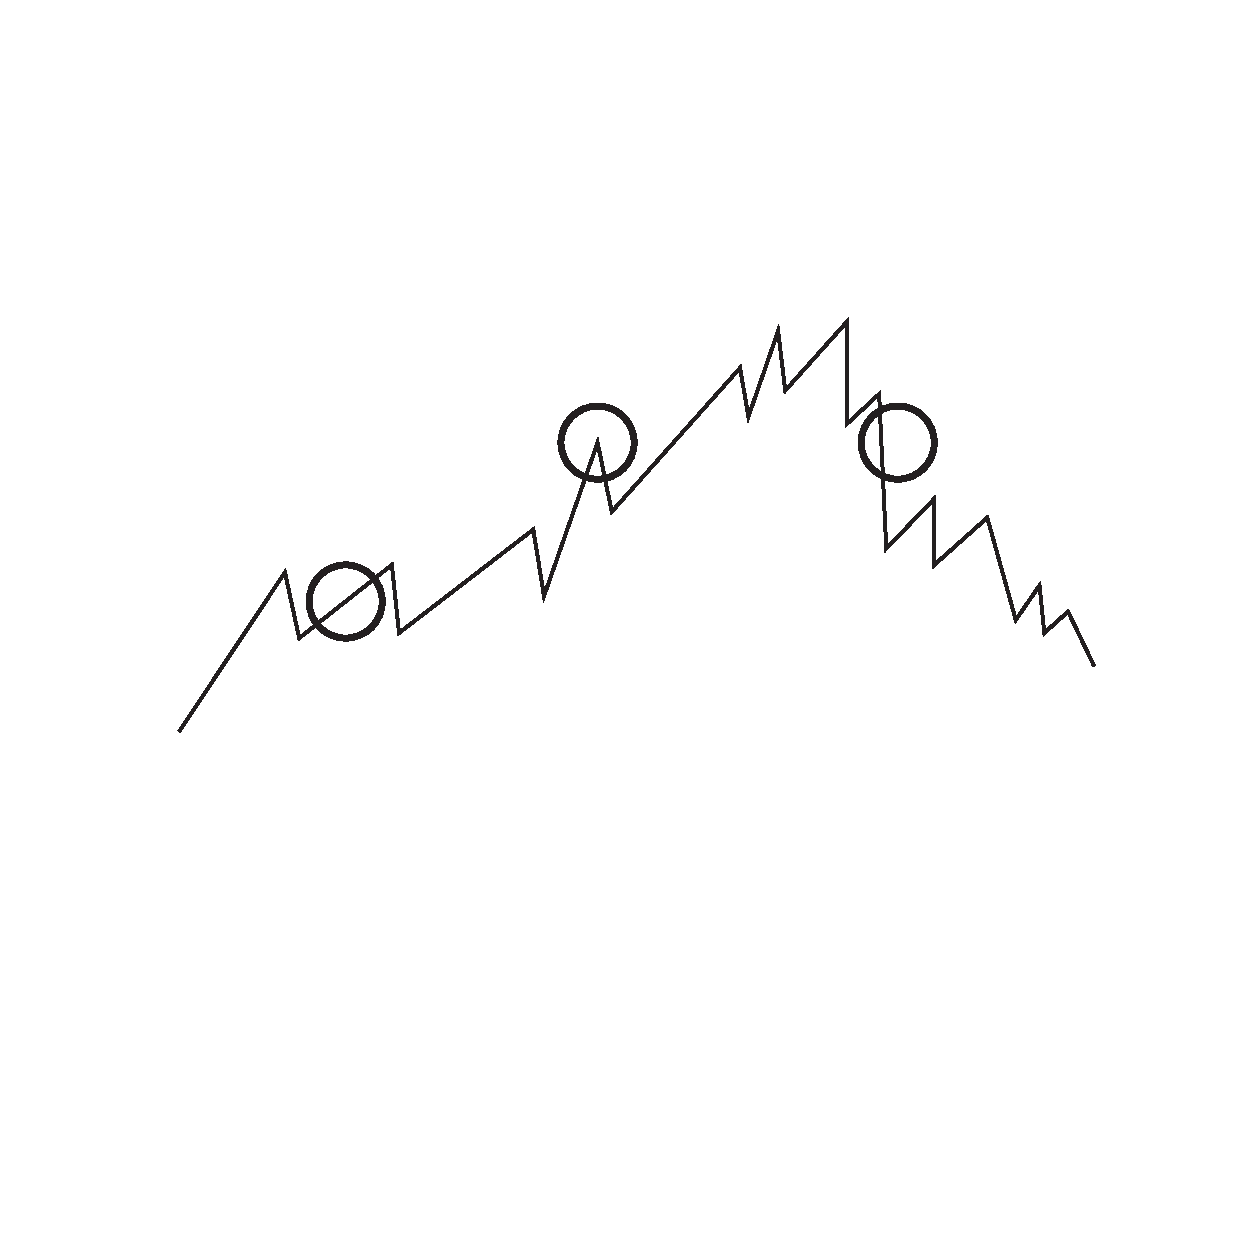
\includepdf[pages=1]{mputo.pdf}
\caption{Metoda prób i błędów}
\centering
\end{figure}
\clearpage

\textbf{Metoda prób i błędów} proponuje nam, abyśmy zgadli wartość $\boldsymbol{x}$ i zapisali związaną z nią wartość $\boldsymbol{y}$. Następnie wielokrotnie powtarzamy fazę zgadywania i zapisu. Po jakimś czasie takiego zgadywania wybieramy $\boldsymbol{x}$ które posiadało związaną z nią najwyższą wartość $\boldsymbol{y}$.\newline

Jest to najprostsza możliwa metoda optymalizacji. Żeby ją stosować, wystarczy utrzymywać w pamięci najlepsze rozwiązanie, na które napotkaliśmy do tej pory i zgadywać kolejne rozwiązania, które mogą być lepsze, czyli najlepiej takie, których poprzednio nie sprawdzaliśmy. Tą metodą możemy sprawdzić każdą możliwą sytuację, jeśli tylko przestrzeń akcji, którą badamy, jest skończona. Mapa, na której szukamy miejsca na dom, powinna być ograniczona np. sąsiadującymi krajami i posiadać ograniczenie małą wielkość kroku. W takiej sytuacji, jeśli damy tej metodzie wystarczająco dużo czasu to doprowadzi nas ona do najlepszego istniejącego rozwiązania. Jest to niewątpliwie silna strona tego podejścia, która pokazuje generalność tej metody. Ta prosta metoda ma jednak również pewne problemy, jak nieskończone przestrzenie powodujące, że wyszukiwanie potrzebuje nieskończonego czasu, aby znaleźć najlepsze rozwiązanie. Także z reguły, czas, który zajmuje ta metoda, w porównaniu do innych jest daleki od najlepszych. Co powoduje taką nieefektywność? Metoda prób i błędów nie posiada żadnej metryki, która pokazywałaby nam, jak bardzo poprawia się nasz wynik w miarę szukania. Można to porównać do szukania przycisku do zapalania światła po omacku. Nie jest to łatwe zadanie, chociaż po pewnym czasie się nam to uda. Sytuację z wyłącznikiem światła poprawia na dodatek fakt, że zazwyczaj wiemy, mniej więcej, w jakim kierunku się on znajduje. Jednak jeśli trafilibyśmy do zupełnie nowego pokoju, to problem ten byłby o wiele trudniejszy. Z takimi trudnościami boryka się metoda prób i błędów. Aby poprawić szybkość szukania, potrzebujemy jakiejś miary, która będzie nam mówić, czy poprawiamy nasz wynik, czy nie. Tak samo gra w szukanie wyłącznika staje się dużo łatwiejsza, kiedy ktoś mówi nam ‘ciepło’ lub ’zimno’ wraz z poruszaniem się po pokoju. Z podobnego rodzaju informacji powinien korzystać nasz algorytm.\newline

\section{Wspinaczka górska}

Pomyślmy, jak moglibyśmy prowadzić nasze poszukiwania, tak aby nie sprawdzać tak wielu złych rozwiązań. Jakiego rodzaju informacji moglibyśmy użyć? Jedną z metod, która mogłaby nam pomóc, jest lepszy wybór punktów do sprawdzenia. Jeśli przestrzeń jest wystarczająco ciągła, to znaczy punkty leżące nieopodal siebie mają podobne właściwości, to moglibyśmy użyć wiedzy o punktach leżących blisko, żeby przybliżać wartość szukanego punktu. Zupełnie jak w grze ciepło-zimno, jeśli wiemy, że jesteśmy w miejscu, w którym niedaleko było ‘zimno’, to prawdopodobnie tu gdzie jesteśmy, też będzie ‘zimno’. Tak więc możemy skupić nasze poszukiwania jedynie na punktach, w których jest ‘ciepło’, czy mówiąc inaczej na punktach, które dają nam dobrą wartość numeryczną funkcji wartości. Ponieważ chcemy prowadzić nasze poszukiwania na dowolnie dużych przestrzeniach, weźmiemy pod uwagę tylko poszukiwanie lokale, czyli takie, które skupia się na wyszukiwaniu optimów lokalnych. Zazwyczaj taki rodzaj poszukiwania ma w danym momencie tylko jednego kandydata na rozwiązanie.\newline

Tu możemy wspomnieć, że istnieją też tak zwane poszukiwania globalne takie, jak np. algorytm mrówkowy, który bierze swoją nazwę od symulowania zachowania owadów, jakimi są mrówki. Tworzy on wiele ‘mrówek’, każda ze swoim osobnym zachowaniem. Akcje poszczególnych mrówek wpływają na siebie tak, że zachowanie całego roju jest bardziej inteligentne niż poszczególnych osobników. Algorytm ten działa na zasadzie zaobserwowanej w świece zwierząt. Mrówki poruszają się po losowych ścieżkach, chyba że znajdą pożywienie. Wtedy wracają do mrowiska, pozostawiając za sobą ślad z feromonów. Inne mrówki napotykając na ślad z feromonów, zaczynają nim podążać, w efekcie samemu wydzielając feromony. W ten sposób uczęszczana ścieżka jest wzmacniana. Kiedy jednak jedzenie się kończy, wydzielanie feromonów zostaje zaprzestane, a ścieżka naturalnie zanika. Podobnego sposobu możemy użyć do znajdywania najlepszych ścieżek na grafie. To nazywane jest poszukiwaniem globalnym, ponieważ próbuje znaleźć globalnie najlepsze rozwiązanie, czyli takie, które jest najlepsze dla całej przestrzeni. Takie poszukiwanie często utrzymuje w pamięci wiele punktów związanych z danym problemem i próbuje znaleźć rozwiązanie, biorąc pod uwagę je wszystkie. W przeciwieństwie do poszukiwania globalnego poszukiwanie lokalne szuka najlepszego rozwiązania tylko w pewnej okolicy. Zazwyczaj utrzymuje też w pamięci informacje o tylko jednym punkcie. Mogłoby się nam wydawać, że poszukiwanie globalne będzie nam bardziej przydatne niż lokalne, jednak najpowszechniej wykorzystywanymi algorytmami w dziedzinie sztucznej inteligencji są algorytmy wyszukiwania lokalnego. To podejście ma jedną ważną korzyść, a mianowicie możliwość użycia informacji o gradiencie. Na razie nie musimy się jednak o to martwić.\newline

O takim sposobie lokalnego poszukiwania możemy myśleć jak o wspinaczce górskiej. Wyobraźmy sobie, że znajdujemy się u podnóża góry, na której szczyt chcemy się wspiąć. Mamy jednak jeden problem. Nie widzimy wierzchołka, gdyż cała góra została pokryta mgłą. Teraz, aby dostać się na szczyt, możemy podjąć następującą metodę działania. Patrzymy się na punkty w widocznej okolicy i wybieramy ten, który znajduje się najwyżej. W jego kierunku się udajemy. Powtarzamy ten proces, dopóki wszystkie punkty znajdujące się obok nas są niżej położone i wtedy stwierdzamy, że znaleźliśmy się na szczycie i kończymy poszukiwania. Oczywiście nie jest powiedziane, że w efekcie działania tej metody znajdziemy się na oczekiwanym szczycie. Może się np. okazać, że wejdziemy na górę znajdująca się obok. Może też się stać tak, że nie wejdziemy na żaden szczyt, tylko utkniemy na pagórku. Ta właściwość tego poszukiwania nazywana jest problemem maksimum lokalnego. Kiedyś uważano, że maksima lokalne są główną przeszkodą w osiąganiu najlepszego rozwiązania. Obecnie poglądy na ten temat uległy zmianie i za najgorsze są uważane płaskie przestrzenie, jednak nie ulega wątpliwości, że możliwym jest utknięcie w maksimum lokalnym. Aby temu zapobiegać, wymyślono metodę losowego resetu (ang. random-restart), która wykonuje wspinaczkę górską wielokrotnie za każdym razem z losowo wybranego stanu początkowego. Ma to służyć omijaniu minimów lokalnych. Jednak wybiegliśmy do przodu, powiedzmy najpierw, czym w ogóle jest algorytm wspinaczki górskiej.\newline

\newpage
\begin{figure}[h]
\includepdf[pages=2]{mputo.pdf}
\caption{Algorytm wspinaczki górskiej}
\centering
\end{figure}
\newpage

\noindent Algorytm \textbf{wspinaczki górskiej} (ang. hill climbing) utrzymuje w pamięci jedno obecnie najlepsze rozwiązanie, sprawdza punkty wokół i porusza się w kierunku największej poprawy wartości, tak długo, jak jakakolwiek może być otrzymana. W tym algorytmie wybór punktów do sprawdzenia odbywa się w pewien specyficzny sposób. Wyobraźmy sobie, że zamiast wybierać najwyższy punkt, sprawdzamy cztery kierunki świata i udajemy się w kierunku, w którym poprawa jest największa. Analogiczne działanie ma algorytm wspinaczki górskiej. W $\boldsymbol{n}$ wymiarach przed zmianą pozycji powinniśmy sprawdzić 2 * $\boldsymbol{n}$ ortogonalnych kierunków. To znaczy kierunków, które znajdują się wobec siebie pod kątem prostym w $\boldsymbol{n}$ wymiarach.\newline

Ten problem tego podejścia wydaje się oczywisty, wraz ze wzrostem ilości wymiarów ilość możliwości, które musimy sprawdzić, rośnie w ogromny sposób. Również niekoniecznie poruszamy się w najlepszym kierunku, ponieważ może on leżeć pomiędzy kierunkami, które sprawdzaliśmy. Wybieramy tylko jeden spośród 2 * $\boldsymbol{n}$
kierunków, który jest najbliżej optymalnego kierunku wchodzenia w górę. Nie użyliśmy też żadnych informacji na temat tak zwanego gradientu.\newline


\section{Metoda gradientu prostego}

Rozmawialiśmy o poruszaniu się w górę zbocza, zwiększając jakąś wartość, ale ludzie ze środowiska optymalizacyjnego z niezbyt jasnych powodów (prawdopodobnie chodzi o jasność notacji) zazwyczaj mówią o poruszaniu się w dół, zmniejszając jakąś wartość. Te pomysły są identyczne poza zmianą znaku. Jeśli konceptualnie odwrócimy przestrzeń na głowie, to możemy zamienić wspinanie się ze schodzeniem w dół i na odwrót.\newline

Mówiliśmy o problemach, jakie są związane z algorytmem wspinaczki górskiej. Głównym problemem jest jednak to, że pomija on pewien rodzaj informacji. Czy możesz wskazać jakiś rodzaj takich informacji, które pozostają nieużyte, a mogłyby nam pomóc? Jednym z problemów jest to, że nie patrzyliśmy się na różnicę między wartością naszej funkcji wartości w poprzednim punkcie a obecnym, żeby znaleźć lepszy kierunek schodzenia. Jak mogłaby nam ta różnica pomóc? Wyobraźmy sobie, że jest ona duża. Oznaczałoby to, że poruszamy się w dobrym kierunku. Jeśli jednak ta różnica jest niewielka, to może powinniśmy się poruszać w innym kierunku, który mógłby nam potencjalnie dać większy zysk funkcji wartości. Teraz weźmy pod uwagę kilka kolejnych kroków i odpowiadające im zmiany funkcji wartości. Chcemy wymyślić sposób wykorzystania tych informacji do wybrania kolejnego kierunku, który będzie potencjalnie najlepszy. Takie połączenie jednych informacji z innymi jest nazywane korelacją. Jeśli mielibyśmy metodę korelacji kierunków, w których poruszaliśmy się z funkcją wartości, to moglibyśmy powiedzieć że kiedy wybierzemy kierunek o historycznie największym spadku to jest to według naszej wiedzy najlepszy kierunek. Taką korelację można znaleźć w bardzo prosty sposób. Wystarczy podzielić zmianę funkcji wartości poprzez wartość kroku w danym kierunku, a później wszystko dodać do odpowiednich kierunków, żeby otrzymać pewne przybliżenie zmiany w każdym kierunku. Następnie wybieramy kierunek o największej historycznej poprawie funkcji wartości. Ponieważ jednak krzywizna przestrzeni będzie się zmieniać, to taka procedura będzie jedynie pewnym przybliżeniem. Najprościej jest jednak założyć, że zmiana w danym kierunku pozostanie taka sama i zachowywać się jak gdyby było to prawdą. Metoda ta może być przydatna nawet w życiu codziennym. Wyobraźmy sobie, że robimy w ciągu dnia różne rzeczy i zapisujemy, jak dobrze czujemy się danego dnia. Później, aby uzyskać ranking rzeczy, które będziemy robić, moglibyśmy rozdzielić to jak dobrze się czuliśmy w proporcjach do tego jak dużo wykonywaliśmy danej czynności dla każdego dnia i dodać wyniki z różnych dni. To dałoby nam numeryczne wartości określające pożądanie danych zachowań, dzięki którym moglibyśmy je uszeregować.\newline

\newpage
\begin{figure}[h]
\includepdf[pages=3]{mputo.pdf}
\caption{Metoda gradientu prostego}
\centering
\end{figure}
\newpage

\noindent Spójrzmy teraz na bardziej matematyczny przykład w 2-dim (dwóch wymiarach):\newline Zaczynamy w punkcie \textbf{\boldsymbol{$p_0$} = (\boldsymbol{$x_0$}, \boldsymbol{$y_0$})} i poruszamy się o wektor \textbf{(1, 2)}. Kończymy w punkcie \boldsymbol{$p_1$} = (\boldsymbol{$x_0$} + 1, \boldsymbol{$y_0$} + 2) albo w innej metodzie zapisu w punkcie \boldsymbol{$p_1$} = (\boldsymbol{$x_1$}, \boldsymbol{$y_1$}). Powiedzmy teraz, że poprawiliśmy naszą funkcję wartości z \textbf{y = \boldsymbol{$y_0$}} do \textbf{y = \boldsymbol{$y_1$}}.\newline

\noindent \textbf{Metoda gradientu prostego} mówi nam, że nasz następny kierunek, w którym będziemy się poruszać, powinien być proporcjonalny do poprawy naszej funkcji wartości (a więc w przykładzie do \textbf{\boldsymbol{$\Delta y$} = y1 – y0}) i także odwrotnie proporcjonalny do kierunku, w którym się poruszaliśmy (więc wektora \textbf{(1, 2)}). W przykładzie następny wektor ruchu będzie równy \textbf{(\boldsymbol{$\Delta y$} / 1, \boldsymbol{$\Delta y$} / 2)} a ogólnie:

\begin{equation}
gradient = \Delta y / \Delta x
\end{equation}

\noindent Gdzie \textbf{gradient} oznacza, ogólnie mówiąc kierunek największego spadku, \textbf{\boldsymbol{$\Delta y$}} to zmiana funkcji wartości, a \textbf{\boldsymbol{$\Delta x$}} oznacza przesunięcie, o które poprzednio się poruszaliśmy.\newline

Co prawda pokazaliśmy przykład działania na gradiencie empirycznym otrzymanym z wykonania kroku optymalizacyjnego, lecz lepszą metodą osiągnięcia tego samego celu jest znalezienie pochodnej funkcji, którą optymalizujemy. Pochodna jest tu sposobem na obliczenie równania (2.2) dla \textbf{\boldsymbol{$\Delta y$}} oraz \textbf{\boldsymbol{$\Delta x$}}, dla których \textbf{\boldsymbol{$\Delta x$}} dąży do zera, a więc intuicyjnie jest to najlepszy kierunek poruszania się dla nieskończenie małego kroku.\newline

\begin{equation}
gradient = f'(x)
\end{equation}

\noindent Gdzie \boldsymbol{$f'(x)$} oznacza pochodną pierwszego stopnia z funkcji \boldsymbol{$f$} w punkcie \boldsymbol{$x$}. Powinniśmy korzystać z tego równania zamiast (2.2) zawsze kiedy umiemy wyznaczyć pochodną\break optymalizowanej funkcji.\newline

Aby otrzymać nowy punkt do sprawdzenia, musimy wziąć informacje o poprzednim punkcie i informacje o gradiencie i przetworzyć je w taki sposób, aby otrzymać
nowy punkt. Najprostszym sposobem na to jest odjąć gradient od starego punktu. Pamiętamy przy tym, że szukamy największego spadku. Jeśli to zrobimy, to otrzymamy tak zwaną formułę rekursywną (co znaczy, że stosujemy ją wielokrotnie na wyniku tej samej formuły) dla znajdywania lepszych punktów:

\begin{equation}
p_{n+1} = p_n - gradient
\end{equation}

\noindent Gdzie \boldsymbol{$p_{n+1}$} jest nowym punktem, z którego będziemy kontynuować poszukiwania, \boldsymbol{$p_n$} jest starym punktem, a \textbf{gradient} jest kierunkiem największego spadku, w którym się poruszamy.\newline

Największym pomysłem, którego tutaj używamy, jest fakt że możemy użyć przeszłej informacji na temat zakrzywienia przestrzeni którą badamy żeby prowadzić nasze wyszukiwania w najlepszym kierunku. Korzystamy z tego, iż niedalekie punkty są często podobne do siebie, np. jeśli jesteśmy w płaskim regionie, to spodziewamy się że jeśli przesuniemy się kawałek dalej to teren nadal będzie płaski. Ten algorytm wraz z pewnymi dodatkami, część, z których zostanie opisana w kolejnych rozdziałach stanowi podstawowy i najczęściej używany algorytm dla optymalizacji w okolicznościach spotykanych w dziedzinie sztucznej inteligencji.\newline

\section{Plus wielkość kroku}

Powiedzieliśmy trochę o wyborze kierunku ruchu, ale nie skupialiśmy się do tej pory na metodach wyboru wielkości kroku. Czytając poprzedni podrozdział, mogłeś myśleć czytelniku, że gradient jest pewnym idealnym krokiem, o który należy się poruszyć niezależnie od sytuacji. Jest prawdą, że gradient podaje nam kierunek największego spadku, lecz nic nie powiedzieliśmy o tym, czy wskazuje on na optymalną odległość. Tak nie będzie. Metody gradientu są więc prawie zawsze, używane wraz z rozwiązaniami, które wybierają wielkość kroku, który mówi nam, jak daleko powinniśmy się przesunąć w kierunku gradientu. Potrzebujemy więc jakiegoś sposobu na określenie wielkości potrzebnego kroku. Najprostszym rozwiązaniem jest dodać do równań pewną zmienną, która będzie określać wielkość kroku. Możemy ją nawet nazwać wielkością kroku. Poprzednie równania zmienią się w następujący sposób:\newline

\begin{equation}
gradient = dy / dx
\end{equation}
\begin{equation}
p_{n+1} = p_n - step\_size * gradient
\end{equation}

\noindent Gdzie równanie (2.4) jest identyczne z równaniem (2.3), a w równaniu (2.5) które jest analogiczne do równania (2.4), pojawia się jednak nowa wartość zwana \textbf{step\_size} czyli wielkość kroku, ta wielkość skalarna będzie nam mówić, jak daleko przesuniemy się za każdym razem.\newline

Należy zaznaczyć, że dodanie wielkości kroku nie zamyka problemu, konieczności odpowiedniego jego wybrania. Teraz możesz się zastanowić, jak powinniśmy dokonać wyboru wielkości kroku. Czy istnieje optymalny sposób na dokonanie tego? Odpowiedź brzmi: Nie, nie ma jednej najlepszej metody wyboru kroku dla każdego problemu. Ta właściwość jest spowodowana faktem, że problemy, które możemy chcieć próbować rozwiązać, mogą być od siebie bardzo różne. Wyobraźmy sobie, że możemy chcieć wspinać się na Babią Górę lub na Rysy, dla każdej z tych gór wielkość kroku, który będziemy robić, będzie inny, dopasowany do nachylenia zbocza oraz ilości przeszkód. Od podobnych czynników będzie zależeć optymalna wielkość kroku w systemach AI. Taka sytuacja jest częsta w tej dziedzinie i jeśli będziesz kontynuował poszerzanie swojej wiedzy o niej, to napotkasz na tę właściwość wielokrotnie. Jedną z rzeczy, która odróżnia fizykę i sztuczną inteligencję jest fakt, że w AI nie ma znanych stałych jak np. \textbf{step\_size} = 0.234… czy coś podobnego. To także oznacza, że ktoś próbujący wytrenować model, na przykład, taki o jakim będzie mowa w rozdziale o sieciach neuronowych, będzie zmieniać taką zmienną, żeby zobaczyć czy poprawia to działanie systemu. Trzeba w tym miejscu zaznaczyć, że takie nudne zmienianie pewnych wartości jest znaczącą częścią pracy kogoś, kto zajmuje się tym zagadnieniem. Ostatecznie, kiedy pewna metoda zostanie opracowana to to, co pozostaje praktyką to dostosowanie jej do swojego konkretnego przypadku, na co zazwyczaj składa się właśnie precyzyjny dobór wielu parametrów. Mimo iż nie ma jednego najlepszego kroku, to istnieją sposoby, które mogą nam pomóc w wyborze takiej stałej. Jak myślisz, w jakim przedziale powinna się znaleźć wielkość kroku? Zwyczajna odpowiedź to gdzieś pomiędzy 0,2 a 0,000001 co jest jednak dosyć dużym przedziałem. Czy możesz pomyśleć o dodatkowej technice, która mogłaby nam pomóc w wyborze kroku? Jednym z istniejących rozwiązań jest tzw. \textbf{planowane zmniejszanie kroku} (ang. learning rate scheduling) Istotą tego podejścia jest zmniejszanie kroku wraz z upływem czasu. Powoduje to dużą eksplorację na początku uczenia i coraz dokładniejsze przeczesywanie najlepszych części przestrzeni pod koniec nauki. Wielkość kroku ma też inną nazwę, a mianowicie \textbf{wskaźnik uczenia} (ang. learning rate), ponieważ wpływa na tempo nauki. Zatrzymajmy się nad tym na chwilę, ponieważ jest to bardzo ważna zależność. Kiedy dokonujemy dużych kroków, to poruszamy się przez przestrzeń szybciej niż gdybyśmy wybrali mniejszy krok, możemy więc powiedzieć, że szybko się uczymy. Nie odbywa się to jednak bez kosztu. Robiąc szybkie postępy, możemy nie zauważyć drobnych niedokładności, jakie mają miejsce przy okazji. Dlatego, gdy postęp zaczyna maleć najlepiej zmniejszyć wskaźnik uczenia i dokonać koniecznych poprawek na mniejszą skalę. W naszym przypadku duży wskaźnik uczenia da nam szybką poprawę, ale może przeskoczyć ponad pewnymi dobrymi miejscami. Za to mały wskaźnik uczenia da nam wolniejszą poprawę, ale sprawi, że nie ominiemy żadnych dobrych regionów. Jedną z metod połączenia tych dwóch korzyści jest planowane zmniejszanie kroku, gdzie wraz z upływem czasu lub po zobaczeniu pewnej ilości przykładów wskaźnik uczenia zostaje pomniejszony. Możemy w pewien sposób myśleć o tym procesie jak o zmniejszaniu temperatury. Przy dużej temperaturze cząsteczka porusza się bardzo gwałtownie, a wraz ze zmniejszaniem temperatury cząstka ogranicza się do dołków energetycznych, czyli regionów gdzie jej energia jest zminimalizowana. Podobny proces możemy zaobserwować w hutnictwie gdzie wyżarzanie, polegające na podgrzaniu i następnym schłodzeniu materiału jest wykorzystywane w celu sprawienia, aby materiał był bardziej podatny dalszej obróbce.

\clearpage
\begin{figure}[H]
\centering
\includepdf[pages=4]{mputo.pdf}
\caption{Wybór wielkości kroku}
\end{figure}
\clearpage

\section{Plus momentum}

Problemem metod gradientu prostego jest to, że często nie jest wydajna. Żeby zobaczyć dlaczego, zastanówmy się nad następującym przykładem. Znajdujemy się w wąskim lekko pochylonym w jedną stronę wąwozie, z dwóch stron mamy strome ściany. Żeby zrobić postęp w takim miejscu, trzeba iść dnem wąwozu, ale wyobraźmy sobie, że znajdujemy się na ścianie takiego wąwozu. Teraz logicznym wydaje się, że trzeba zejść na dno i iść dnem takiego wąwozu. Zobaczmy jednak, jak zachowuje się algorytm gradientu prostego w takiej sytuacji. Jak myślisz, co będzie wynikiem jego działania? Odpowiedź brzmi: algorytm gradientu prostego będzie się poruszał w kierunku przeciwnym do kierunku biegu wąwozu, ponieważ jeśli jest on odpowiednio wąski, to będziemy przeskakiwać od razu na przeciwną ścianę. Kiedy już znajdziemy się na przeciwnej ścianie to podobnie, w następnej iteracji, przeskoczymy z powrotem na ścianę, z której zaczęliśmy. Żeby zobaczyć, dlaczego tak się dzieje, pomyśl, w jakim kierunku porusza się algorytm gradientu prostego. Porusza się on zawsze w kierunku największego gradientu, inaczej mówiąc w kierunku największego spadku. Dla ściany wąwozu największy spadek jest w dół wąwozu, a nie w kierunku biegu wąwozu. Niestety nie będziemy się poruszać w kierunku prawdziwej poprawy wartości, a raczej tymczasowej, która zostanie wymazana poprzez następujący za chwilę niechybny powrót na ścianę, z której zaczynaliśmy. Nasza droga będzie przypominać powolne zygzakowanie w poprawnym kierunku. Pochyłość wąwozu sprawi co prawda, że będziemy się poruszali w dobrą stronę, ale będzie to bardzo powolny postęp. Żeby zapobiegać takiemu niekorzystnemu zjawisku wprowadzono pęd (ang. momentum).\newline

\clearpage
\begin{figure}[H]
\centering
\includepdf[pages=5]{mputo.pdf}
\caption{Zachowanie optymalizatora bez dodatku pędu}
\end{figure}
\clearpage

\noindent W fizyce pęd jest zdefiniowany jako:

\begin{equation}
R = m * v
\end{equation}

\noindent Gdzie $\boldsymbol{R}$ oznacza pęd, $\boldsymbol{m}$ masę a $\boldsymbol{v}$ prędkość.\newline

\noindent Siła zdefiniowana jest jako:

\begin{equation}
F = d(mv) / dt
\end{equation}

\noindent A więc jest pochodną pędu po czasie.\newline

\noindent Teraz wiedząc, że siła jest zmianą pędu, wyobraźmy sobie, że czas podzielony jest na małe części. Wtedy, żeby dostać pęd w n-tym kroku, należałoby obliczyć wartość następującego rekursywnego równania:

\begin{equation}
R_{n+1} = R_{n} + F
\end{equation}

\noindent Ponieważ $\boldsymbol{F}$ jest zmianą w $\boldsymbol{R}$.\newline

\noindent Jest jeszcze jeden mały szczegół, którego nie bierzemy pod uwagę. W prawdziwym świecie obserwujemy tarcie, które sprawia, że każdy ruch traci swój pęd w miarę upływu czasu. To tarcie nazwiemy $\boldsymbol{\alpha}$ i będzie ono opisywać procent pędu, który nie jest wytracany w jednym kroku czasu. Równanie zmienia się następująco:

\begin{equation}
R_{n+1} = \alpha * R_{n} + F
\end{equation}

\noindent To jest równanie na pęd w metodzie gradientu, jeśli tylko podstawimy odpowiednie wartości za $\boldsymbol{R}$ i $\boldsymbol{F}$. Przypomnijmy sobie teraz równanie służące do znajdywania lepszych punktów (2.5):

\begin{equation}
p_{n+1} = p_{n} - step\_size * gradient
\end{equation}

\noindent Teraz, zamiast używać zmiany \textbf{step\_size} * \textbf{gradient} zastąpmy ją pędem.

\begin{equation}
p_{n+1} = p_{n} + R_{n+1}
\end{equation}

\noindent Następnie rozwińmy $\boldsymbol{R_{n+1}}$ przy pomocy równania (2.9):

\begin{equation}
p_{n+1} = p_{n} + \alpha * R_{n} + F
\end{equation}

Jak mówiliśmy, musimy podstawić odpowiednie wartości. Pęd $\boldsymbol{R_n}$ zastąpimy zmienną, która będzie oznaczać zmianę wartości punktu $\boldsymbol{p_n}$ dla poprzedniej iteracji. Jednak ta zmiana jest zależna od drugiej części równania ($\boldsymbol{\alpha} * \boldsymbol{R_n}$ + $\boldsymbol{F}$), które opisuje tę zmianę, więc jak możemy zauważyć pęd $\boldsymbol{R_{n+1}}$ będzie zależny od siebie samego w poprzedniej iteracji. Tak więc musimy utrzymywać w pamięci drugą część równania, aby użyć go ponownie w następnej. Za to $\boldsymbol{F}$ które w fizyce jest zmianą w pędzie, zastąpimy zmianą zmiany wartości punktu czy inaczej zmianą pędu dla punktu. $\boldsymbol{F}$ będzie więc równe gradientowi, który będzie określał tę zmianę tak, aby pęd zbliżał się do optymalnego pędu. Równanie (2.9) ze zmienionymi zmiennymi prezentuje się następująco:

\begin{equation}
\Delta p_{n+1} = \alpha * \Delta p_n - gradient
\end{equation}

\noindent A równanie (2.12) otrzyma ostateczną formę:

\begin{equation}
p_{n+1} = p_n - gradient + \alpha * \Delta p_n
\end{equation}

\noindent Gdzie $\boldsymbol{p_n}$ jest wartością wyszukiwania w n-tej iteracji, \textbf{gradient} jest gradientem, $\boldsymbol{\alpha}$ jest parametrem ‘tarcia’, a $\boldsymbol{\Delta p_n}$ określa zmianę w $\boldsymbol{p_n}$ dla poprzedniej iteracji. Tu znowu $\boldsymbol{\alpha}$ jest stałą, którą możemy zmieniać, bo nie ma dla niej jednej najlepszej wartości dla każdego problemu. Wszystko co następuje po minusie jest identyczne jak prawa strona równania (2.13) określającego nasz pęd.\newline

Zauważmy jeszcze jedną rzecz, która mogła cię zaniepokoić. Przed gradientem postawiliśmy znak minus. Wynika to z tego, że gradient określa kierunek największego wzrostu funkcji. Ponieważ my chcemy ją minimalizować, to powinniśmy się udać w przeciwnym kierunku. Jeśli jeszcze kiedyś zaniepokoisz się znakiem, to pomyśl czy nie wynika to właśnie z tej zależności. Wracając do metafory wąwozu, równanie (2.13) sprawia, że będąc w wąskim przesmyku, będziemy dodawać poprzedni pęd do obecnego. Będą się one nawzajem niwelować, ponieważ będą skierowane w przeciwnych kierunkach, a to, co zostanie, będzie kierowało nas w dół wąwozu, wygładzając naszą podróż.\newline

\section{SGD}

W rozdziale dotyczącym gradientu prostego ukryliśmy jedną ważną informację. Chodzi nam tu o sposób obliczania gradientu. Aby obliczyć gradient, potrzebujemy pewnego przykładu, który da nam przestrzeń, nad którą będziemy mogli optymalizować nasz punkt. Jednak często spotykamy się z sytuacją, gdy nie chcemy dopasować naszej wartości do jednego przykładu, ale jest tych przykładów więcej. Pomocny w tym procesie jest zbiór danych.\newline

\clearpage
\begin{figure}[H]
\centering
\includepdf[pages=6]{mputo.pdf}
\caption{mini-batch SGD}
\end{figure}
\clearpage

\noindent \textbf{Zbiór danych} jest kolekcją pewnych danych, które mają ze sobą coś wspólnego. Np. możemy mówić o zbiorze zdjęć ze ślubu lub o zbiorze nazw książek na twojej półce albo o zbiorze cen pewnych produktów.

\begin{equation}
D = [x_1, x_2, x_3, …]
\end{equation}

Możemy sobie wyobrazić sytuację, w której chcielibyśmy, powiedzmy znaleźć najlepsze położenie nie tylko dla naszego domu, ale też dla wybudowania całego osiedla mieszkaniowego. Musimy wtedy wziąć pod uwagę preferencje wszystkich naszych klientów, a nie tylko nasze własne. Używając zbioru danych, moglibyśmy przechowywać preferencje dla wszystkich klientów. Aby zrobić jeden krok naszego algorytmu gradientu prostego, musielibyśmy obliczyć gradient, używając wszystkich przykładów ze zbioru danych, więc liczba obliczeń wzrosłaby proporcjonalnie do wielkości zbioru danych. W tym wypadku gradient dla pojedynczego kroku byłby sumą gradientów dla każdego przykładu. Możesz sobie wyobrazić, że może to być dość niepraktyczne, jeśli zbiór składa się z tysięcy, a nawet milionów przykładów. Jak rozwiązać ten problem, zmniejszając liczbę koniecznych obliczeń, a jednocześnie zachowując generalizację? Rozwiązaniem jest tu wykonanie pojedynczego kroku z jednym przykładem, a następnie przejście do innego przykładu i wykonanie kroku już na nim. Tym sposobem w pewnym momencie korzystamy z informacji na temat każdego przykładu, jednocześnie oszczędzając na obliczeniach. Właściwie takie podejście nazywa się \textbf{metodą gradientu stochastycznego} (ang. stochastic gradient descent) a krótko SGD. Algorytm ten otrzymuje swoją nazwę od tak zwanej stochastyczności, czyli matematycznej nazwy na procesy losowe. W tym przypadku nazwa związana jest z losowością powstającą na skutek używania pojedynczych przykładów, które mogą być niereprezentatywne dla całego zbioru danych. Widzimy więc, że SGD ma też swoje wady. Jakie są główne różnice pomiędzy używaniem całego zbioru danych a używaniem pojedynczego przykładu? Trenowanie na całym zbiorze danych jest dokładniejsze, ponieważ różnice między pojedynczymi przykładami się niwelują, ale jest również bardziej kosztowne obliczeniowo. Natomiast używanie pojedynczego przykładu przeciwnie: jest mniej kosztowne obliczeniowo, ale za to dużo bardziej niedokładne. Może więc moglibyśmy znaleźć rozwiązanie, tak aby spotkać się w połowie drogi. Trenujmy na kilku przykładach wybranych z naszego zbioru danych. To podejście nazywa się \textbf{mini-batch} co z angielskiego oznacza „mały pakiet”. Algorytm nazywa się mini-batch SGD. Czasami dla skrótu mówi się na niego SGD, opuszczając pierwszy człon, co może być mylące dla osoby niezaznajomionej z tematem. Takie podejście zniweluje fluktuacje w funkcji wartości, które możemy obserwować w czystym SGD i sprawi, że uczenie będzie łatwiejsze. Ten algorytm jest jednym z najczęściej stosowanych w AI. Nawet pomimo tego, że był on jednym z pierwszych, które zostały wymyślone, to nadal jest często używany i potrafi osiągnąć najlepsze wyniki w trenowaniu np. sieci neuronowych.